% thesis.tex

\documentclass[12pt]{report}

\usepackage{utepcsthesis}
\usepackage{graphicx}

\usepackage{amsmath}
\usepackage{amsfonts}
\usepackage{bm}

\usepackage{algorithmicx}
\usepackage{algorithm,algpseudocode}



\DeclareMathOperator*{\argmin}{\arg\!\min}
\DeclareMathOperator*{\argmax}{\arg\!\max}
\begin{document}

\graphicspath{{Diagrams/}}
%%%%%%%%%%%%%%%%%%%%%
% Preliminary Pages %
%%%%%%%%%%%%%%%%%%%%%%%%%%%%%%%%%%%%%%%%%%%%%%%%%%%%%%%%%%%%%%%%%%%%%%%%%%%%%%%%

% Set the table of contents depth (tocdepth) to the least significant section
% type that you want to be included in the table of contents using this key:
%   1 = section
%   2 = subsection
%   3 = subsubsection
%   4 = paragraph
\setcounter{tocdepth}{2}

% The graduate school requires all caps for the title, and if
% the title contains more than one line, the lines should be
% of decreasing length, giving the look of an inverted pyramid.

\title{ANALYSING THE EFFECTS OF DATA AUGMENTATION AND HYPER-PARAMETERS FOR TEXT CLASSIFICATION WITH CONVOLUTIONAL NEURAL NETWORKS}
% If the title is more than one line, separate the lines with \\[1pc]
% as shown below:
%\title{THIS IS THE VERY FIRST LINE\\[1pc]
%       THIS IS THE SECOND LINE\\[1pc]
%       THIS IS THE THIRD ONE}

% The author should also be all caps
\author{JONATHAN K. QUIJAS}
% Uncomment to put degrees on title page
%\AuthorDegrees{B.S.}
\date{May 2017}
\DeptName{Department of Computer Science}

\CommitteeChair{Olac Fuentes, Chair, Ph.D.}
\CommitteeMembers{Monika Akbar, Ph.D.}
                 {David Novick, Ph.D.}
%Uncomment if you have a fourth member on your committee
%\AdditionalMember{Additional Member's name}

\GradSchoolDean{Charles Ambler, Ph.D.}

%Produce the signature page
\makesigpage

%Uncomment if you want a copyright page
\begin{CenteredPage}
\copyright Copyright\\[0.2in]
by\\[0.2in]
Jonathan K. Quijas\\[0.2in]
2017
\end{CenteredPage}

%Delete if you don't want a dedication
\begin{CenteredPage}
{\it to my\\[0.2in]
FAMILY\\[0.2in]
thanks for everything}
\end{CenteredPage}

\maketitlepage

% acknowl.tex {Acknowledgements}

\addcontentsline{toc}{chapter}{Acknowledgements}

\chapter*{Acknowledgements}
       % Acknowledgements, optional
%\include{preface}       % Preface, optional
% abstract.tex (Abstract)

\addcontentsline{toc}{chapter}{Abstract}

\chapter*{Abstract}
Convolutional neural networks have seen much success in computer vision natural language processing tasks.
Because of the large number of parameters in these model's, they are prone to overfitting
if not regularized appropriately or trained on a sufficiently large dataset.
In this work, we study the performance of convolutional neural models when the available training datasets
are of moderate size. We quantify the effects of model hyperparameters on classification performance
and propose several data augmentation techniques designed for text datasets.
Finally, we provide discussion on our empirical results.
      % Abstract, optional, but strongly recommended

\tableofcontents        % Generate Table of Contents
\listoffigures

% If you a list of tables, uncomment the next line.
% It is required if the document contains three or more tables
%\listoftables

% If you use a list of figures, uncomment the next line
% It is required if the document contains three or more figures
%\listoffigures

% Here would go optional list of illustrations, maps, slides

%%%%%%%%
% Body %
%%%%%%%%%%%%%%%%%%%%%%%%%%%%%%%%%%%%%%%%%%%%%%%%%%%%%%%%%%%%%%%%%%%%%%%%%%%%%%%%

%Start arabic numbering, bottom of first page and top right of subsequent pages
\StartBody

% chap1.tex {Introductory Chapter}

\chapter{Introduction}

\section{Brief Overview of Deep Neural Networks}
Deep convolutional neural networks have seen an enormous amount of success on a wide array of application, from
scene interpretation to self-driving vehicles and art generation[CITE]. Natural language processing tasks are no exception to the
range of problems deep learning can solve, from sentiment analysis to language modeling. In this work, we focus our efforts to studying
convolutional and recurrent neural networks for text classification. Especifically, we analyse how well modern neural networks models performed
using scientific abstract text data from multiple disciplines such as astro-physics and computer science.

\section{Training a Neural Network}

A neural network is a function $f(\bm{x};\bm{\theta})$ that maps its input $\bm{x}$ to some response variable $y$. When we \textit{train} a
neural network, we \textit{learn} the model parameters, or weights, $\bm{\theta}$ that minimize some cost function $J(\bm{\theta})$.
For a regression task, where the model's output is a continuous variable, a common cost function is the \textbf{Mean Square Error}:
\[J(\theta) = \frac{1}{m}\sum_{i=1}^{m}(y_{i} - f(\bm{x}_{i};\bm{\theta}))^{2}\]

For categorical or discrete output variables found in e.g. classification tasks, we use the \textbf{Categorical Cross-Entropy}:

\[J(\bm{\theta}) = -\mathbb{E}_{\bm{x},y \sim \hat p_{data}} \log \textit{p}(y|\bm{x};\bm{\theta})\]

Given a \textit{training} set of observations $\bm{x}_i$ and their true labels $y_i$, we compute weights that minimize the cost, or error, via
maximum likelihood (ML) estimation:

\[\bm{\theta}_{ML} = \argmax_{\bm{\theta}} \sum_{i}^{m} \log P(y_{i}|\bm{x}_{i};\bm{\theta})\],

which one can see is the equivalent of computing the weights that \textbf{\textit{minimize}} the cross-entropy cost function.


%\section{Minimizing Non-Convex Functions: Gradiant-Based Learning}
%Convex functions are easy to optimize. Their global minimum is guaranteed and any local minimum is a global minimum. This means that when a
%procedure optimizes a convex function, its solution is truly optimal[CITE]. Said procedure is also guaranteed to converge from any initial point in parameter space[CITE].
%Due to the non-linearities associated with a neural network, the loss function to be minimized becomes non-convex.
%[Elaborate (Weight symmetry, model identifiability, etc)]

%Because of the non-convexitivity of neural network optimization, we usually rely on gradient-based methods. This involves iteratively \textit{moving},
%or updating, the values of our weights in the direction opposite of the cost function's gradient. These updates should be small, scaled by a
%\textit{learning rate}, and can make learning a lengthy process. Nonetheless, this method is effective and allows for learning of a good
%set of weights, although in practive it is rarely the optimal[CITE].

\section{Bias-Variance Tradeoff}
When learning a neural network's weights, we use a \textit{training set} so that we can later generalize
previously unseen data with high accuracy (or some other determined metric). That means that during training, we
obtain $\bm{\theta}_{ML}$ by minimizing $J_{train}(\bm{\theta})$, but we care about having low $J_{test}(\bm{\theta})$ i.e. low cost
on test data points.

\textbf{Overfitting} occurs when a network is able to predict its training set extremely well i.e. very close to zero error, but fails to predict
unseen data points. This is because the network's weights have been extremely fine-tuned to \textit{fit} its training data, but do not fit or represent
data points outside of its training sample.
An overfitted model is said to have large \textbf{variance} and small \textbf{bias}. Conversely, underfitting occurs when the model fails to predict
the training set because it generalizes too harshly. This model is said to have large bias and small variance.

Because of the commonly large amount of weights in deep convolutional networks, it is easy to overfit even a moderate size training set[CITE].
Many techniques exist to avoid overfitting in a neural network
[EXPAND]

In this work, we study the effects of multiple regularization techniques used to avoid overfitting in a neural network[REFER TO CHAPTER].


-Describe and cite conv nets for text classification
-Describe the conv net pipeline
-Add figure of pipeline
-Comment that LSTM have made huge progress
-Describe difficulty with smaller datasets
Convolutional neural networks obtain state of the art results on image and text processing tasks.


\section{Data Augmentation: Increasing Training Sample Size}
-Describe usual augmentation schemes for vision tasks
-describe why they work, small changes, same class
-propose augmentation scheme and refer to corresponding chapter
         % Introductory Chapter
% chap2.tex (Definitions)

\chapter{Text Classification with Deep Neural Networks}\label{TXT-CLASS}

\section{Brief Overview of Deep Learning}
Deep convolutional neural networks have seen much success on a wide
array of application, from scene interpretation to self-driving vehicles and art generation.
Natural language processing tasks are no exception to the range of problems
deep learning can solve, from sentiment analysis to language modeling. One very useful function of deep neural networks
is their ability to learn high-level features at each consecutive layer \cite{le2013building}.

One type of neural networks that is particularly good at learning features from the data is the convolutional neural network (CNN)\cite{lecun1989backpropagation}\cite{oquab2014learning}\cite{dosovitskiy2014discriminative}.
A CNN learns a set of weights, or kernels, that are normally much smaller than the input size.
The difference in size forces the weights to have \textbf{sparse interaction}, or interaction on a subregion of the input, versus the dense interaction
between every input with every output in traditional neural networks (i.e. vector-matrix multiplication). This sparse interaction
allows for features to be detected locally within the input (e.g. edge detection).
\textbf{Parameter sharing} allows for distinct outputs to be computed using the same set of weights. This drastically reduces
the number of unique weights and allows for significant increases in network depth (i.e. deep networks) without the need
to increase the amount of training data.
These two design principles make CNN's poweful and efficient feature extractors.

Another type of deep neural network that has seen much success is the recurrent neural network (RNN). RNN's are designed to model data that display temporal structure, such as text and speech. By \textit{unfolding}
time-steps as a computational graph, the network can learn to model data along the time dimension, using at each time step the
raw input plus the output of the last time step's layer [Siegelman and Sontag 1995]. Because of the usually very deep structure of
the recurrent network, computation of the gradient via back propagation can lead to the \textit{vanishing gradient} problem, where the gradient
starts to shrink and become very close to zero as we back-propagate the errors. \cite{hochreiter1997long} proposed
the \textbf{Long Short-Term Memory (LSTM)} recurrent network, a type of recurrent that essentially solves this problem with recurrent networks.
A recent and simpler variation of the LSTM network is the Gated Recurrent Unit (GRU), which performs comparably well \cite{chung2014empirical}.



\section{Word Embeddings}
Another significant achievement of deep learning for natural language processing is the neural probabilistic language model. \cite{bengio2003neural}
proposed a neural network to model the probability of a word given its context
$P(w_t|w_{t-k},\dots,w_{t-1})$

In their work, they addressed the curse of dimensionality, manifested by the fact that a test word sequence $(w_{t-k},\dots,w_{t})$
is likely to be different from all training sequences, by learning distributed representations of words. Words are represented as
dense continuous vectors called \textbf{word embeddings}.
Using word embeddings to model the likelihood of word sequences allowed generalization because the language model
would give high probability to unseen word sequences if they were made up of words semantically similar to already seen words.
Because of the of the underlying algorithm used to learn these word embeddings, similar words tend to lie closer to each other on
embedding space. Thus, word embeddings are said to capture semantic relations and encode more information than just a word identifier (e.g.
a bag-of-words or one-hot vector representation).

\begin{figure}[h]
\caption{Visualization of embeddings using the t-distributed stochastic neighbor embedding (t-SNE) dimensionality reduction algorithm.
Words with similar or related meanings tend to lie close to each other in embedding space.}
\centering
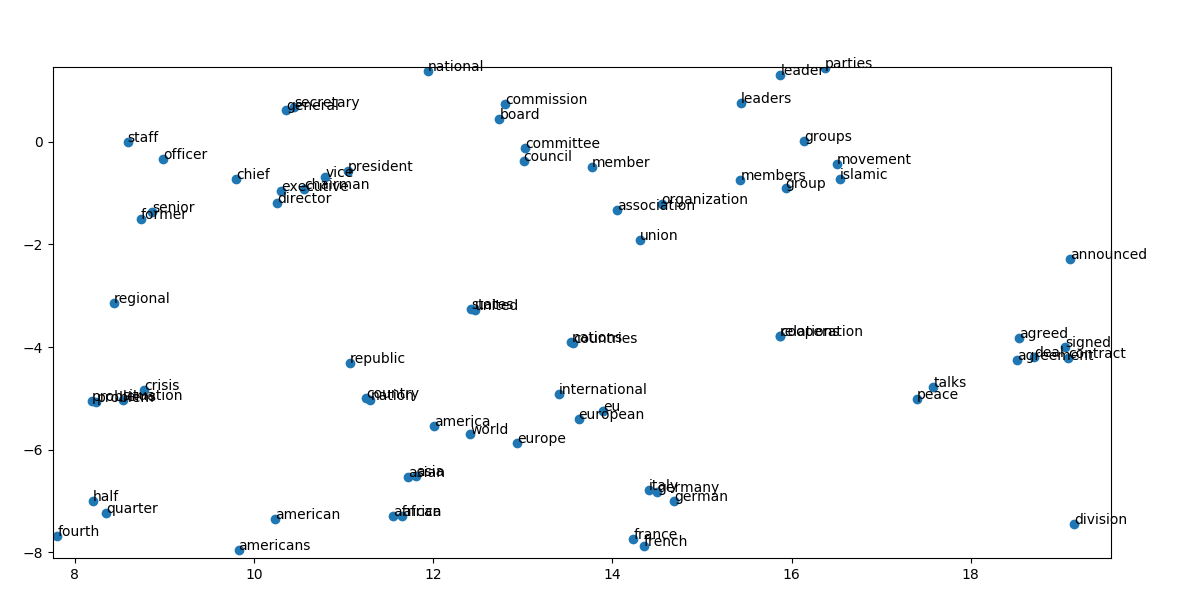
\includegraphics[width=1.0\textwidth]{EmbeddingViz.png}
\end{figure}

\section{Convolutional Neural Networks}
As described previously, convolutional neural networks are known for their abilities to learn high-level features from raw data. As input signals advance
forward through the network, they produce latent signals as linear conbinations with learned parameters, have non-linearities applied
to them, and have a pooling or selection mechanism based on simple functions such as the average or maximum operations \cite{zhou1988image}.

When dealing with image data, images are convolved with multiple filters, each convolution applied to overlapping subimages called as receptive fields.
This localized convolution process leads to discovery of low level features of images in the training set such as edges. As data
flows forward through the model, higher level features are discovered (e.g. wheels or headlights in a vehicle image dataset).

These convolutional neural networks are comprised of \textit{feature maps}. A feature map is a \textbf{convolution} layer paired with a
\textbf{pooling} layer afterwards. The convolution stage creates \textit{activations}, whereas the pooling stage
reduces dimensionality and creates translation invariance.


\subsection{Input Representation: Word Embeddings for Convolutional Networks}
We can take advantage of word embeddings to apply convolutions to text in a fashion similar to convolutions with
image data and exploit the semantic information in the embeddings \cite{kim2014convolutional}. We apply the convolutions to overlapping sub-regions of the input text i.e. bi-grams, tri-grams, etc.
After convolution, we apply a non-linear function such as $max(0,x)$ and reduce data dimensionality
by pooling such as $x_{pool} = max(x_1,\dots,x_n)$.
Given a set of documents $\bm{s_1},...,\bm{s_m}$, we build a vocabulary $\mathbb{V}$ and a bag-of-words model from $\mathbb{V}$ to create a mapping $BoW:\mathbb{V} \mapsto \{1,...,|\mathbb{V}|\}$.
We represent a training document $\bm{s}$ as a sequence of integers $BoW(\bm{s})=$ $\bm{x} = x_1,...,x_k$, each integer being simply a word index
in $\mathbb{V}$. When the convolutional network receives this input sequence, each word index will be mapped to a corresponding embedding vector.

\begin{figure}[H]
\caption{Visualization of a feature map with a single kernel. In this example, the kernel convolves tri-grams, or windows of three words.
After convolution with all possible trigram context windows, max pooling is applied to reduce dimensionality.
Here, the pool size is 3. This process is repeated as many times as there are kernels in the layer and their outputs are
concatenated horizantally to yield a matrix of size \textit{num filters} $\times$ (\textit{input length - pool size + 1}).}
\centering
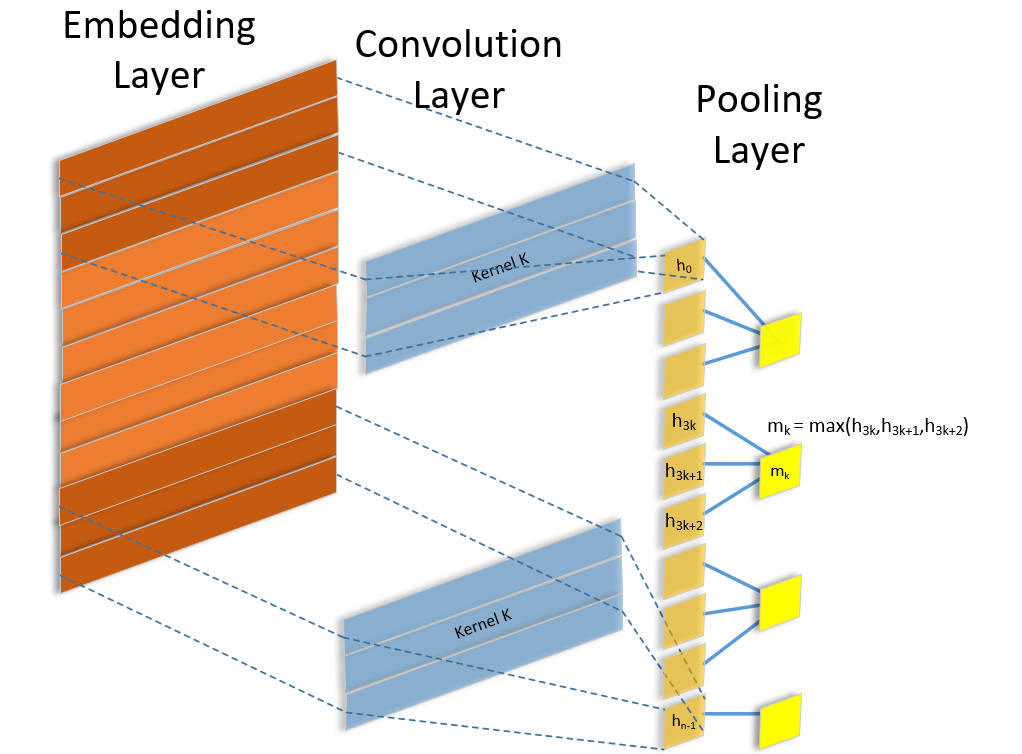
\includegraphics[width=0.5\textwidth]{FeatureMap.png}
\label{fig:convolution}
\end{figure}
%%% Local Variables:
%%% mode: latex
%%% TeX-master: "thesis"
%%% End:
         % Chapter 2
% chap4.tex (Definitions and Theorem)

\chapter{Model, Dataset, and Final Pipeline Description}
\section{Model Description}
A standard architecture for convolutional neural networks for text sequence classification is an embedding layer
followed by a feature map and a dense layer with a softmax activation to output class probabilities, as proposed by \cite{kim2014convolutional}.
\begin{figure}[H]
\centering
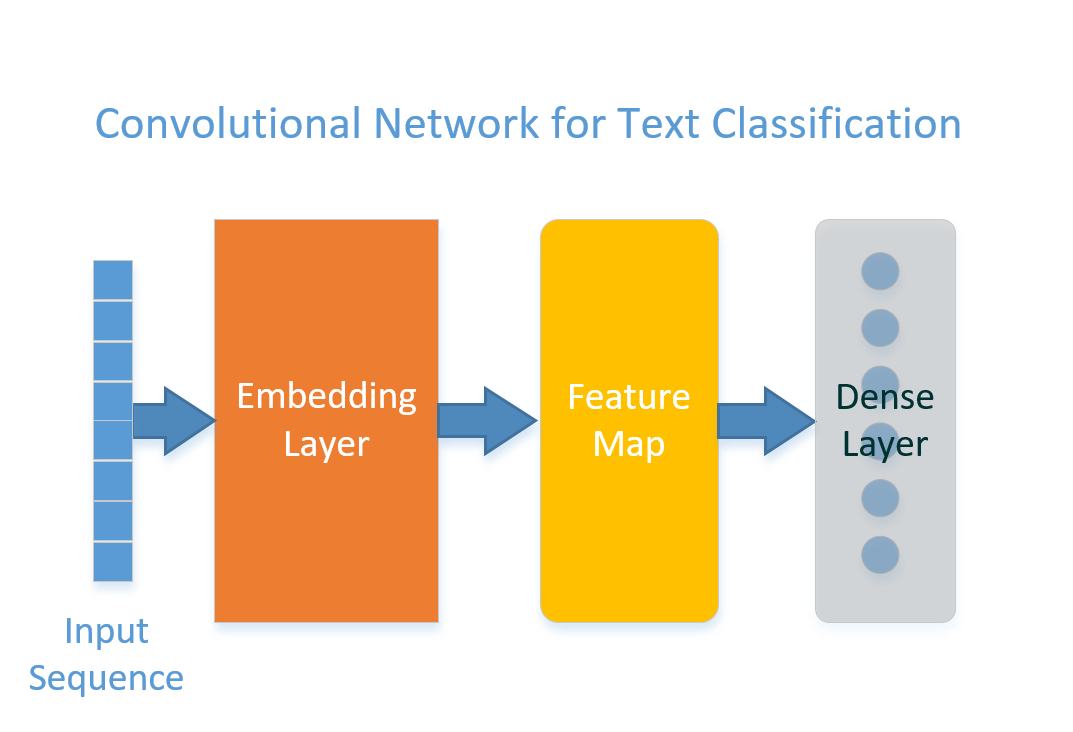
\includegraphics[width=0.5\textwidth]{ConvText.png}
\caption{A common architecture for a convolutional network for text classification is an embedding layer followed by a feature map, then a
dense layer to compute class probabilities.}
\end{figure}
This model has parameter sharing and sparse interaction properties inherent of convolutional
neural networks, and thus is a good choice for efficiently extracting features from the data via convolutions and non-linearities.
The pooling operation acts as a feature selection mechanism and reduces the number of outputs in its layer. This reduction makes forward propagation
an even more efficient process. Convolutional neural networks, however, are not designed to consider the data as having temporal
structure, as is the case with text sequence data.


Another popular neural model for text classification is the recurrent neural network. This architecture is explicitly designed to treat
data that display temporal structure. Because of this, the recurrent neural network is an excelent choice for text sequence data.
At a basic level, this architecture is comprised of an embedding layer (to transform input sequences into word embeddings)
followed by a recurrent layer, then a dense layer with the softmax activation to output probabilities.
In the following sections we provide a technical description of the model layers introduced above.
A more in-depth description of typical neural models used for natural language processing is presented by \cite{yin2017comparative}.
\section{Layer Descriptions}
\subsection{Embedding Layer}\label{embeddinglayer}
The \textbf{embedding layer} layer is usually the first layer in a convolutional neural network that processes text input for classification tasks.
Given an input sequence of words $\bm{s}=\{w_1,\dots,w_n\}$, we transform it into a sequence of indexes $BoW(\bm{s})=$ $\bm{x} = x_1,...,x_n$.
The embedding layer maps each index $x_i$ to a corresponding embedding and outputs an embedding matrix $\mathbf{E} \in \mathbb{R}^{n \times d}$, where $d$ is
the embedding size. These embeddings may be further fine-tuned during training. Because of the large number of
parameters in this layer (number of words allowed times embedding size), it is usually a good idea to
use $L_2$ regularization or dropout in order to avoid or mitigate overfitting.

\begin{figure}[H]
\centering
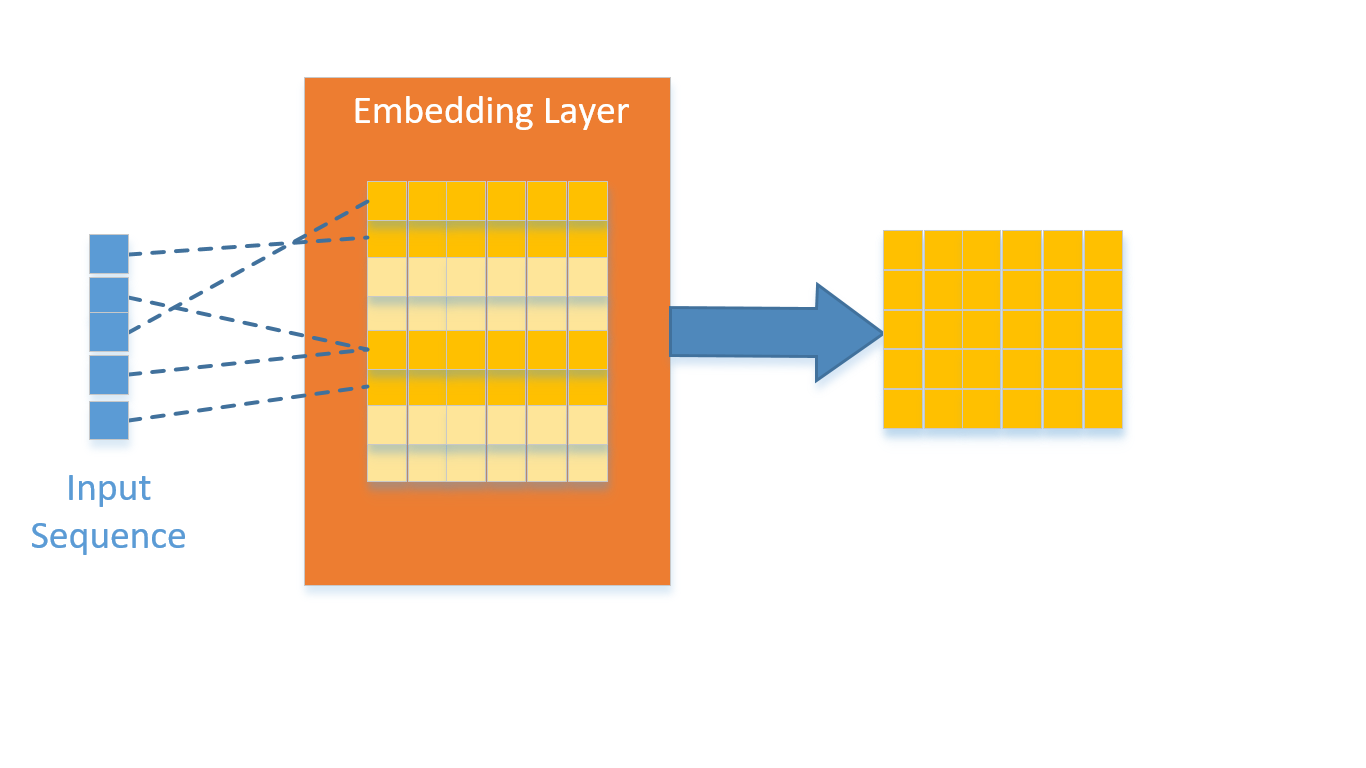
\includegraphics[width=0.5\textwidth]{EmbeddingLayer.png}
\caption{Visualization of an embedding layer. Word indexes are mapped to word embeddings via table lookups. This
layer outputs a matrix comprised of stacked embeddings, one for each index.}
\end{figure}

\subsection{Feature Maps: Convolution + Pooling}

We refer to a convolutional layer followed by a pooling layer as a feature map.
Since our data are text sequences with temporal structure, we use a one-dimensional convolutional
layer to convolve with embedding n-grams through the input sequence \cite{waibel1988phoneme}.
As in Figure \ref{fig:convolution}, we stride only along the time-dimension. This is in contrast to the usual two-dimensional convolution schemes with image data,
where the kernels stride along the width and height dimensions of the input data. Concretely, the convolution between the $i$th word embedding
vector $\bm{w}_i$ and a kernel $\bm{k}$ is given by:
\[\bm{s}(i) = \sum_{j=1}^{d}\bm{w}_i(j)\bm{k}(j)\],

where $d$ is the embedding size.

After the convolution step,
we apply a non-linearity to each computed feature. We chose the rectified linear activation (\textbf{ReLU}) function
\[ReLU(x) = max(0,x)\]
Although simple, this non-linearity is quite effective and thus widely used.
We then use a max pooling operation
\[maxpool(\bm{x}) = \max_i{ \bm{x} }\]
to ouput a single value for each kernel as done in to \cite{DBLP:journals/corr/LinCY13}.
Max pooling is a strong feature selection and dimensionality reduction mechanism.
We pass to the next layer the single strongest activation from each kernel.

\subsection{Gated Recurrent Unit Layer}
A recurrent layer is designed to process data with temporal structure\cite{rumelhart1986sequential}.
This recurrent layer is in itself a network, where the hidden layer values at time \textit{t} depend on the previous
hidden layer's values, the input corresponding to time \textit{t}, and a shared parameter set:
\[\bm{h}^{t} = f(\bm{h}^{t-1}, \bm{x}^{t}, \bm{W}, \bm{V})\]
This is implemented by \textit{unrolling} the layer along the time dimension as a sequence of layers, each corresponding
to a moment in time. Because of this design, back-propagation of error through the unrolled layer can result
in the vanishing gradient problem (i.e. the gradients shrink exponentially as they propagate backwards through the network layers).

\begin{figure}[H]
\centering
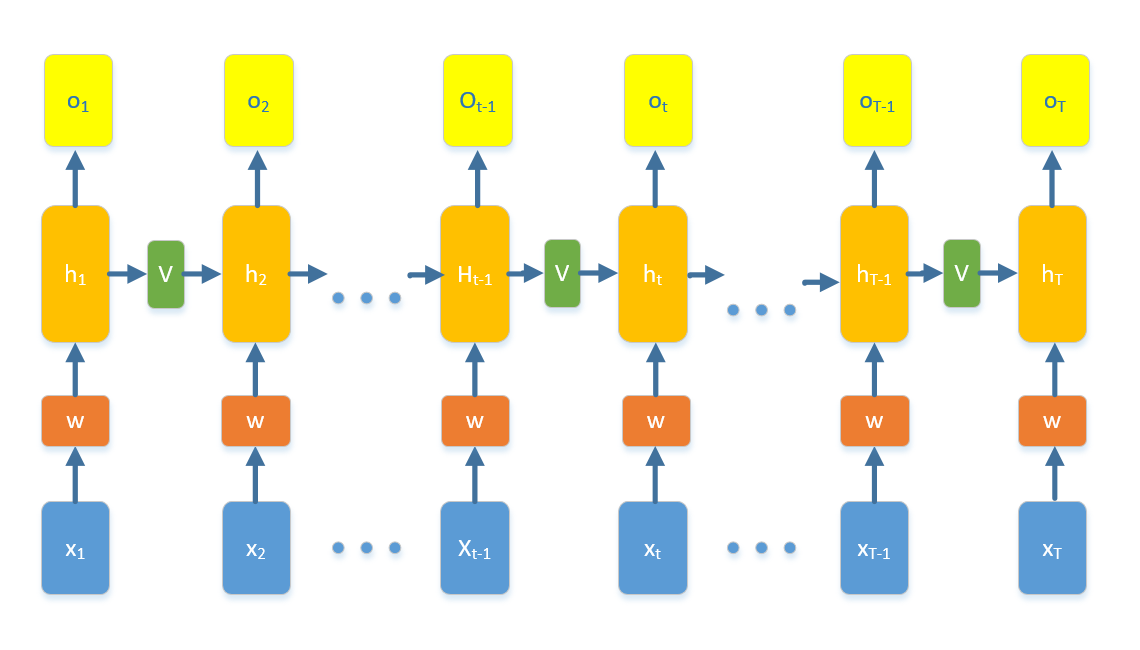
\includegraphics[width=0.5\textwidth]{RecurrentNet.png}
\caption{Visualization of a recurrent layer. Each hidden layer $\bm{h}^{\textit{t}}$ is a function of the previous hidden
layer $\bm{h}^{\textit{t-1}}$ and the present input signal $\bm{x}^{\textit{t}}$. The weights are shared across time steps
in order for the model to generalize better.}
\end{figure}

A Gated Recurrent Unit layer is a type of recurrent layer designed to combat this condition \cite{chung2014empirical}.
It is a simplified version of the earlier LSTM layer \cite{hochreiter1997long}, also designed to mitigate the vanishing gradient problem.
In practice, this type of recurrent layer normally performs as well as its more complex predecesor.
This layer models the latent features computed by the feature map as a time sequence. This means that it
does not assume indepencies between computed activations and learns to model the temporal structure of the previous
layer's output. This property makes the layer an adequate choice for text sequence data.

\subsection{Dense Layer}
The last layer in our model is the classical \textbf{dense}, or fully connected layer.
The number of units in this layer is equal to the number of classes in our dataset.
Given the output of the network's second to last layer $\bm{h}$, we can compute the unnormalized log probabilities
\[\bm{z} = \bm{\theta}^{T}\bm{h} + \bm{b}\]
where $\bm{b}$ is the bias vector.



Each  $z_i$ is a log probability of the input corresponding to class $i$. The \textbf{softmax} activation function is then applied to
all the units, to finally output class probabilities:

\[\hat{y}_i = softmax(\bm{z})_i = \frac{e^{z_i}}{\sum_j e^{z_j}}\],
\[\hat{y}_i = P\{y=i|\bm{x}\}\]

In our experiments, a purely convolutional neural network finished training in a significantly shorter amount of time compared to the recurrent network.
Because of the convolution and pooling operations, the CNN normally processed the data around 10 times faster than the RNN. The RNN, although slower,
always achieved around 4\% higher accuracy on all experiments.

After testing both architectures, the model we use in the rest of this work is a mixture of these two standards.
After the embedding layer, we add a feature map to extract features from the raw inputs,
then we add a GRU layer. This design choice incorporates the sequence modeling power of the RNN with the fast and efficient feature extraction of the CNN.
This combination always led to the highest accuracy achieved with the RNN, with the reduced training times of the CNN. Out of all the features computed by a kernel, we select only the single strongest one
(i.e. highest value). The pooling layer's output size is therefore equal to the number of kernels in our convolutional layer. In order to create
a one-to-one correspondance between the network's inputs (the word indices in the input sequence) and the units in the recurrent layer, we chose to have
a number of kernels equal to the network's input size (i.e. length of input sequence).
This design choice proved to be very efficient and reached the highest accuracy percentages during our experiments.

\begin{figure}[H]
\centering
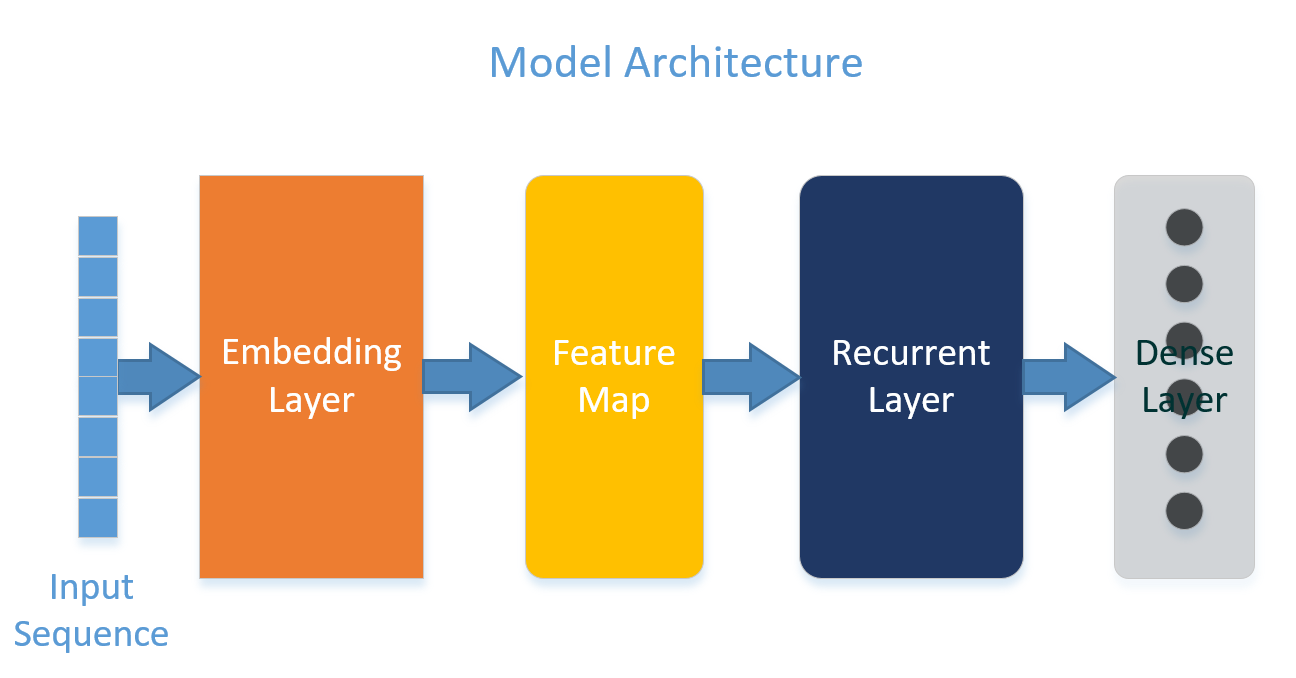
\includegraphics[width=0.5\textwidth]{ModelPipeline.png}
\caption{Model Architecture: embedding layer, followed by a feature map, and a recurrent layer. At the end, we have
a fully connected layer with a softmax activation, which will output class probabilities.}
\end{figure}

The final network's architecture is as follows:
\begin{itemize}
  \item Input layer: word index vector
  \item Embedding layer: maps word index vector to embedding matrix
  \item Feature Map:
      \begin{itemize}
        \item Convolution layer: kernel size=5, \textit{ReLU} activation
        \item Global MaxPooling layer: Outputs a scalar per kernel
      \end{itemize}
\item Gated Recurrent Unit layer with \textit{tanh} activations
\item Dense layer with \textit{softmax} activations
\end{itemize}
         % Chapter 3
% chap3.tex (Definitions and Theorem)

\chapter{Towards Improving Model Performance: Embeddings and Data Augmentation}
As mentioned in [REFER TO SECTION], we can fine-tune the word embeddings via back-propagation and gradient descent (or some other
gradient-based optimizer), just as any other weights in the neural network. In this case, the number of parameters in our model increases drastically.
With more free parameters to learn from the data, it is easier to overfit. This is especially true if the amount of training data is limited, as is the case
with our particular task. Another important aspect to consider when fine-tuning the embeddings is whether we lose the semantic information originally
present in them. It is therefore a good idea to quantify the effect of training the embeddings. In the following sections, we propose different ways
treat the embedding layer in our neural network in order to mitigate overfitting. We also consider reducing the dimensionality of the embeddings
via Principal Component Analysis (PCA). Finally, we propose data augmentation techniques inspired from computer vision tasks but designed for
text data with temporal structure, as is the case with our data.

\section{Freezing the Embedding Layer}
When we make our model's embeddings trainable, its number of parameters highly increases. With inputs of size $n$,
and embeddings of size $d$, we introduce $n \times d$ new parameters into the model.
We therefore propose multiple embedding \textit{trainability} schemes to quantify how much the embeddings help increase (or decrease) test
accuracy and overfitting.

\begin{itemize}
  \item{Frozen Embeddings}
  \begin{itemize}
    \item{With this scheme, we \textit{freeze} the embedding layer altogether. Not once during training do we update
    the embedding vectors, so the model relies completely on its other parameters to fit the data.}
  \end{itemize}
  \item{Freeze-Unfreeze}
  \begin{itemize}
    \item{With the \textit{freeze-unfreeze} scheme, we train the model with its embedding layer frozen until some
    stopping criterion is met e.g. early stopping due to validation error increase. After this, we \textit{unfreeze}, or make the
    embedding layer trainable, and retrain the model.}
  \end{itemize}
  \item{Flash-Freeze}
  \begin{itemize}
    \item{In the \textit{flash-freeze} scheme, we allow the embedding layer to be trainable for a small number of
    epochs e.g. two, then freeze it and retrain the model.}
  \end{itemize}
  \item{Unfrozen Embeddings}
  \begin{itemize}
    \item{We allow the embeddings layer to be trainable from the very beggining. We consider this training scheme as our \textbf{baseline}.}
  \end{itemize}
\end{itemize}

\section{Principal Component Analysis and Dimensionality Reduction of the Embeddings}
Principal Component Analysis (PCA) is a very popular linear transformation commonly used to reduce dimensionality of a dataset CITE[Shlens 2005].
It projects the data to a representation where each variable is linearly uncorrelated. Concretely, PCA rotates the data onto new axes called principal
components. Given a data matrix $\bm{X}$ with $n$ dimensions, its principal components are the eigenvectors of the covariance matrix $\bm{X}^T\bm{X}$. The first principal component is the direction of most variation. The second principal component is the direction with the next largest amount
of variation, and so on. We can then choose to retain only the $k<n$ principal components that contain the most amount of variation in the data.

We propose to apply PCA to the word embeddings in order to linearly decorrelate their dimensions and reduce their dimensionality.
By reducing the dimensionality while preserving the majority of the variance in them (e.g. 95\%), we will reduce the amount of parameters introduced
to the model while retaining most of the information from the original embeddings.



\section{Dataset Augmentation: Shuffling and Noise Injection}
Another common practice aimed to reducing overfitting is to \textbf{augment} the dataset.
Data augmentation refers to any transformation of the input data in a way that
the label value does not change. Data augmentation is ubiquitous in computer vision tasks. Example transformations include translations,
rotations, and color intensity jitters via Pricipal Component Analysis CITE[krizhevsky 2012]. All these tranformations should be subtle enough that the overall structure is preserved, but
allow for the model to process more distinct training data points.

The data augmentation techniques mentioned above are common practive in computer vision tasks such as image classification.
In order to introduce more variance into our dataset, we propose data augmentation techniques inspired by computer vision by designed for
text sequence data.
We propose to \textbf{shuffle} by randomly changing the order of words within a \textbf{context windows}, or non-overlapping neighborhood of words
in the input text sequence.
We further propose to inject small amounts of \textbf{noise} to the input sequence by randomly replacing words with words taken from the training vocabulary.

As long as the overall structure of the data (and label) is preserved, data augmentation normally lead to improved task performance CITE[Chawla et al 2002]
CITE[Krizhevsky et al 2012]CITE[Simonyan and Zisserman 2015] CITE[He et al 2016].
With that same rationale, we expect our proposed augmentation techniques to yield increase accuracy percentages. In other words, we expect that
our changes will be subtle enough for the label to be preserved, but effective enough that we introduce more variance into our dataset and help cope with
the limited amount of training examples.


\subsection{Shuffling}
We propose to augment our dataset by making small \textit{context} changes that don't change the global structure
of the input sequences. Concretely, we move a \textit{context window} along non-overlapping neighborhoods the input sequence, randomly
shuffling the words indexes inside it. For example using a context window of size 2 i.e. \textit{bi-gram}, an input sequence
\[\bm{x} = x_1, x_2, x_3, x_4, x_5, x_6\]

 could be shuffled to:
\[\bm{x}^{\prime} = x_2, x_1, x_3, x_4, \underbrace{x_6, x_5}_\text{bi-gram}\]
In the first pass, the first two indexes get shuffled. The second pass led to no changes in ordering. The third and
final pass shuffles the last two indexes.

As it is common practice in computer vision tasks to apply small translations and rotations to images, we perform
this operation to slightly perturb the temporal structure of our text sequence data.
The rationale for this dataset augmentation technique is that small changes in the ordering of the words will
result in a larger training sample; a training input sequence has a low chance of being repeated as its
length increases. Smaller context windows preserve the most structure. This method will preserve
most of the original context structure in the sequence, as long as the shuffling is not to harsh e.g.
a complete random permutation of the sequence.

\subsection{Noise Injection}
One common augmentation technique for image datasets is to add small amount of noise. By replacing a relatively small
amount of pixel values with noise, the model gets to process and train on a different but similar instance. The noise should be subtle
enough as to not distort the image too much, otherwise we could potentially train the model using mostly noise.
We propose to augment our dataset by injecting small amounts of noise to each training sample. Again, we aim to simulate
a larger training sample while avoiding harsh changes to the original inputs. Concretely, each word in a text sequence gets replaced
with a specified probability with a word randomly chosen from our training vocabulary.
\begin{algorithm}[H]
\caption{Add noise to input sequence}
\begin{algorithmic}[1]
\Procedure{NoiseInjection}{$\bm{x}=[x_1,...,x_n], \mathbb{V}, p_{noise}$}
\For {$k$ = 1 to $n$}
\If{$p_k \sim \textit{U}(0,1) \leq p_{noise}$}
\State$x_k \gets x^{\prime}_k \in \mathbb{V}$
\EndIf
\EndFor

\Return $\bm{x}$
\EndProcedure
\end{algorithmic}
\end{algorithm}


\section{Dataset Augmentation: Padding}

Although more complex neural models are designed to cope with variable length input,
in practice a more common and simple approach is to pad data to be of some specified
length as described in chapter [CITE CHAPTER].
In order to enforce uniform input size for our neural networks,
we apply \textbf{zero-padding}.For any arbitrary training instance $BoW(\bm{s})=$ $\bm{x} = x_1,...,x_k$, we enforce that $k = n$, for the specified input size
$n$. Thus, if $k \textless n$, we transform it into $\bm{x}_{pad} = x_1,...,x_k, 0_{k+1}, ..., 0_{n}$. Conversely, if
$k \textgreater n$, we simply truncate $\bm{x}$ to be of size $n$. The input length introduces another model hyper-parameter
that should be fine-tuned, but a reasonable approach is to pad enough to fully accomodate
the length of most input sequences i.e. it’s preferrable to pad than truncate and lose
information.

Our network's input is a sequence of integers, each integer being a word index: a number representing a word in our vocabulary $\mathbb{V}$.
Word indexes range from 1 to $|\mathbb{V}|$, and the index 0 being left for out-of-vocabulary words.
When we pad our input sequence with 0’s, we don’t add any additional information; we
simply create a constant input length. We propose that if instead we add values that characterize or help
describe the input sequence more thoroughly, we may increase the amount of useful information
available during neural network training.

Consider a very simple input sequence, and assume its true label can be determined
from a single word:

\[\text{"This paper is about computer graphics"}\]

where the label is "Graphics" i.e. a publication about computer graphics.
In this simple case, the label is determined by the word "graphics". To the human reader, this single informative word
is enough for the classifier to predict the label correctly although it is only 1/6 of the entire text.

Now consider a the padded version, where we enfore an input length of 10:

\[\text{"This paper is about computer graphics PAD PAD PAD PAD"}\]

In the padded version, the word graphics is now only 1/10 of the entire text. If we
could pad the sequence using this informative word instead of some
meaningless token e.g. 0's, we could increase the likelihood of the model extracting features from it. In other
words, make important words be present more frequently.
We propose to pad input sequences with values found already within the
input text sequence instead of 0's only.

\subsection{Wrap Padding}
Our proposed padding scheme is to \textit{wrap around} the text, repeating words once we reach the padding portion.
Refering back to the first example, the input sequence:
\[\text{"This paper is about computer graphics PAD PAD PAD PAD"}\]

would then be
\[\text{"This paper is about computer graphics This paper is about"}\]

One thing to observe is that using this simple scheme, we remove all 0's i.e. non-informative padding indexes
from the text sequence, but we also don't have selection mechanism and can miss useful words such as missing the
word "\textit{graphics}" in this example. Nonetheless, it is a simple approach to pad our data and increase the likelihood of encountering informative
words during feature extraction.


\section{Reducing Data Granularity: From Abstract to Sentences}
Our last proposed dataset augmentation scheme is break each training abtract into a set of sentences, and train
the network using this finer text granularity. For example, training a model using single sentences, another using sentence pairs,
and another using sentence triplets.
During testing, we break a test abstract into sentence sets and classify each set individually. We then assign
the class with the largest mean.
         % Chapter 4
% chap5.tex (Definitions, Theorem and Proof)

\chapter{Experimental Results} \label{Results}
In this chapter we will show our results.

\section{Dataset Descriptions}

We scraped a scientific publication abstract dataset from Arxiv.org. Concretely, we gathered
publications from the physics, mathematics, computer science, quantitative biology,
and quantitative finance departments. For each department, we considered each \textbf{topic} as a
class. For example, when considering computer science publications, we considered the
"computational complexity" topic as one class, "artificial intelligence" as another class,
and so on. We apply simple preprocessing to the texts by removing non-alphanumeric
characters, and converting to lower case characters.

\begin{center}\begin{tabular}{||c c||}
 \hline
 Department & Number of Labels\\ [0.5ex]
 \hline\hline
AstroPhysics & 5\\
Physics & 13\\
Computer Science & 20\\
Mathematics & 26\\
Quant. Bio & 0\\
 [1ex]\hline\end{tabular}\end{center}

For our pretrained embeddgins, we used the GloVe embedding set [CITE GLOVE]. This set consists of six billion tokens, each represented
as a vector of size 100.

\section{Freezing the Embeddings: Results}
We tested the four different proposed embedding training approaches.
The first is to leave the embeddings frozen throughout training i.e. non-trainable parameters.
The second approach is to freeze the embeddings until convergeance, then retrain with the embeddings unfrozen.
The thid approach is to train with the embeddings unfrozen for a small amount of epochs e.g. three, then
freeze the embeddings and retrain the model.
The last approach is to simply train with the embeddings as trainable parameters from the very beggining.

We now present our results
\begin{center}\begin{table}[H]\begin{tabular}{||c c c c c c ||}
 \hline
 Dataset & Training Set Size & Frozen & Not-Frozen & Freeze-Unfreeze & Flash-Freeze\\ [0.5ex]
 \hline\hline
AstroPhysics & 17500 & .755(6) & .770(8) & 0.769(14) & \textbf{.775(6)}\\
Physics &  45000 & .715(9) & \textbf{.781}(10) & .777(39) & .780\textbf{(8)}\\
Computer Science & 63400 & .621\textbf{(9)} & .693(12) & 0.695(56) & \textbf{.701}(10)\\
Mathematics & 87700 & .590(22) & \textbf{.685}(21) & .678(72) & .684\textbf{(11)}\\
Quant. Bio & 11000 & .834(15) & .835(6) & 0.836(21) & \textbf{.841(5)}\\
 [1ex]\hline\end{tabular}\caption{Accuracy results on all datasets with proposed embedding training schemes.
 The numbers in parenthesis represent the number of epochs until the model converged.}
\end{table}\end{center}

We observe that the Flash-Freeze method achieves relatively faster convergence, with accuracy competent or better than
the accuracy of all other methods.

\section{Data Augmentation Results}
In this section we show our experimental results when using our proposed data augmentation techniques. Our model hyper-parameters are as follows:
number of training words=20000, kernel size=3, learning rate=0.001, regularization rate=0.00001,
dropout rate = 0.2, maximum sequence length = 250.

%
%%%%%%%%%%% ASTROPHYSICS
%
\section{AstroPhysics}
[Distribution]
\subsection{Baseline}
\begin{center}\begin{tabular}{||c c c c c c c c c||}
 \hline
 NWords & Batch & MaxLen & $p_{drop}$ & Kern & Pool & $\alpha$ & $\lambda$ & Acc\\ [0.5ex]
 \hline\hline
 30000 & 64 & 200 & 0.442 & 3 & 5 & 1e-3 & 1e-4 & 0.773\\
 \hline
 80000 & 64 & 250 & 0.059 & 3 & 2 & 1e-4 & 1e-5 & 0.760\\
 \hline
 80000 & 64 & 250 & 0.056 & 2 & 2 & 1e-3 & 1e-4 & 0.759\\
 [1ex]\hline\end{tabular}\end{center}

\subsection{Padding}
\subsubsection{Wrap Padding}
\begin{center}\begin{tabular}{||c c c c c c c c c ||}
 \hline
 NWords & Batch & MaxLen & $p_{drop}$ & Kern & Pool & $\alpha$ & $\lambda$ & Acc\\ [0.5ex]
 \hline\hline
 30000 & 64 & 200 & 0.442 & 3 & 5 & 1e-3 & 1e-4 & 0.773\\
 \hline
 80000 & 64 & 250 & 0.059 & 3 & 2 & 1e-4 & 1e-5 & 0.761\\
 \hline
 80000 & 64 & 250 & 0.056 & 2 & 2 & 1e-3 & 1e-4 & 0.760\\
 [1ex]\hline\end{tabular}\end{center}

\subsubsection{CSO Padding}
\begin{center}\begin{tabular}{||c c c c c c c c c ||}
 \hline
 NWords & Batch & MaxLen & $p_{drop}$ & Kern & Pool & $\alpha$ & $\lambda$ & Acc\\ [0.5ex]
 \hline\hline
30000 & 64 & 200 & 0.442 & 3 & 5 & 1e-3 & 1e-4 & 0.774\\
\hline
80000 & 64 & 250 & 0.059 & 3 & 2 & 1e-4 & 1e-5 & 0.752\\
\hline
80000 & 64 & 250 & 0.056 & 2 & 2 & 1e-3 & 1e-4 & 0.761\\
 [1ex]\hline\end{tabular}\end{center}

\subsubsection{LSH Padding}
\begin{center}\begin{tabular}{||c c c c c c c c c ||}
 \hline
 NWords & Batch & MaxLen & $p_{drop}$ & Kern & Pool & $\alpha$ & $\lambda$ & Acc\\ [0.5ex]
 \hline\hline
 30000 & 64 & 200 & 0.442 & 3 & 5 & 1e-3 & 1e-4 & 0.768\\
 \hline
 80000 & 64 & 250 & 0.059 & 3 & 2 & 1e-4 & 1e-5 & 0.752\\
 \hline
 80000 & 64 & 250 & 0.056 & 2 & 2 & 1e-3 & 1e-4 & 0.755\\
 [1ex]\hline\end{tabular}\end{center}


\subsection{Sentence Split}
\subsubsection{Mean Vote}
\begin{center}\begin{tabular}{||c c c c c c c c c ||}
 \hline
 NWords & Batch & MaxLen & $p_{drop}$ & Kern & Pool & $\alpha$ & $\lambda$ & Acc\\ [0.5ex]
 \hline\hline
 30000 & 512 & 50 & 0.395 & 3 & 3 & 1e-5 & 1e-4 & 0.730\\
 \hline
 60000 & 512 & 40 & 0.051 & 4 & 4 & 1e-5 & 1e-6 & 0.7152\\
 \hline
 20000 & 512 & 40 & 0.062 & 5 & 5 & 1e-4 & 1e-6 & 0.685\\
 \hline
 20000 & 512 & 60 & 0.247 & 3 & 5 & 1e-3 & 1e-5 & 0.710\\
 \hline
 10000 & 512 & 60 & 0.121 & 5 & 3 & 1e-3 & 1e-5 &  0.712\\
 \hline
 70000 & 512 & 40 & 0.223 & 4 & 5 & 1e-5 & 1e-5 &  0.690\\
 \hline
 40000 & 128 & 50 & 0.225 & 5 & 3 & 1e-5 & 1e-4 &  0.734\\
 \hline
 30000 & 64 & 40 & 0.132 & 3 & 4 & 1e-3 & 1e-4 &  0.711\\
 \hline
 40000 & 1024 & 50 & 0.225 & 5 & 3 & 1e-4 & 1e-4 &  0.689\\
 [1ex]\hline\end{tabular}\end{center}

\subsection{Noise Injection}
\begin{center}
 \begin{tabular}{||c c c c c c c c c c c||}
 \hline
 NWords & Batch & MaxLen & $p_{drop}$ & Kern & Pool & $\alpha$ & $\lambda$ & $p_{aug}$ & $p_{noise}$ & Acc\\ [0.5ex]
 \hline\hline
 80000 & 64 & 250 & 0.548 & 4 & 5 & 1e-4 & 1e-5 & 0.653 & 0.195 & 0.537\\
 \hline
 70000 & 64 & 300 & 0.423 & 5 & 4 & 1e-5 & 1e-3 & 0.107 & .004 & 0.665\\
 \hline
 70000 & 32 & 200 & 0.512 & 3 & 4 & 1e-3 & 1e-5 & 0.179 & .373 &  0.764\\
 \hline
 80000 & 128 & 200 & 0.185 & 4 & 4 & 1e-5 & 1e-6 & 0.973 & 0.128 &  0.680\\
 \hline
 50000 & 32 & 250 & 0.167 & 4 & 4 & 1e-4 & 1e-4 & 0.866 & 0.364 & 0.761\\
 [1ex]\hline\end{tabular}\end{center}




%
%%%%%%%%%%% MATH
%
\section{Math}
[Distribution]
[Distribution]
\subsection{Sentence Split}
\subsubsection{Mean Vote}

\subsection{Padding}
\subsubsection{Wrap Padding}
\begin{center}\begin{tabular}{||c c c c c c c c c c ||}
 \hline
 NWords & Batch & MaxLen & $p_{drop}$ & Kern & Pool & $\alpha$ & $\lambda$ &  Loss & Acc\\ [0.5ex]
 \hline\hline
 80000 & 64 & 250 & 0.548 & 4 & 5 & 1e-4 & 1e-5 & 1.818 & 0.537\\
 \hline
 2 & 7 & 78 & 5415 \\
 [1ex]\hline\end{tabular}\end{center}

\subsubsection{CSO Padding}
\begin{center}\begin{tabular}{||c c c c c c c c c c ||}
 \hline
 NWords & Batch & MaxLen & $p_{drop}$ & Kern & Pool & $\alpha$ & $\lambda$ &  Loss & Acc\\ [0.5ex]
 \hline\hline
 80000 & 64 & 250 & 0.548 & 4 & 5 & 1e-4 & 1e-5 & 1.818 & 0.537\\
 \hline
 2 & 7 & 78 & 5415 \\
 [1ex]\hline\end{tabular}\end{center}
\subsubsection{LSH Padding}
\begin{center}\begin{tabular}{||c c c c c c c c c c ||}
 \hline
 NWords & Batch & MaxLen & $p_{drop}$ & Kern & Pool & $\alpha$ & $\lambda$ &  Loss & Acc\\ [0.5ex]
 \hline\hline
 80000 & 64 & 250 & 0.548 & 4 & 5 & 1e-4 & 1e-5 & 1.818 & 0.537\\
 [1ex]\hline\end{tabular}\end{center}

\subsection{Noise Injection}
\begin{center}
 \begin{tabular}{||c c c c c c c c c c c c||}
 \hline
 NWords & Batch & MaxLen & $p_{drop}$ & Kern & Pool & $\alpha$ & $\lambda$ & $p_{aug}$ & $p_{noise}$ & Acc\\ [0.5ex]
 \hline\hline
 80000 & 64 & 250 & 0.548 & 4 & 5 & 1e-4 & 1e-5 & 0.653 & 0.195 & 1.818 & 0.537\\
[1ex]\hline\end{tabular}\end{center}
         % Chapter 5
% chap6.tex (Significance and Future Work)

\chapter{Conclusions}
We presented an evaluation of recurrent convolutional neural networks for classification of publication abstracts from multiple science and
engineering disciplines. We proposed techniques that resulted in a small increase in test accuracy compared to our baseline model.

One conclusion we can make from this study is that recurrent convolutional networks are efficient and effective feature extractors even with
moderate amounts of training data. The combination of convolution and global max pooling provided efficient feature extraction, while the recurrent layer
learned to model the temporal structure of our data. The model with this combination of layers reached the highest test accuracy in our experiments.

We proposed several embeding \textit{trainability} schemes to manipulate the word embeddings during training.
The results we obtained were different than what we had anticipated. Since the embeddings were already learned (pre-trained) from a previous task
using a very large dataset to represent words in a distributed way and to capture semantic relations,
we originally believed that changing their values would only overfit the training set and thus significantly reduce testing set accuracy.
We expected that the \textit{freeze-unfreeze} method would achieve faster convergeance and higher accuracy compared to all other proposed embedding methods.
With this scheme, we hoped the model would converge then increase accuracy by allowing the embeddings to be trainable until convergeance determined by
a stopping criterion. Although the model test accuracy did increase with this scheme, the \textit{flash-freeze} method outperformed all others.
By allowing the embeddings to be fine-tuned for a small number of iterations (three in our tests), then allowing the model to rely
only on its weights (frozen embeddings), we observed we could finish training after a constant number of epochs.
For our task, three epochs were enough to finish training. Not only did the \textit{flash-freeze} method achieve the highest overall performance, but it also
removed the need for a validation set to use for early termination.
This increased, albeit by not much, the amount of data available for training purposes since we could stop training after a constant number of epochs.
A validation set for early stopping was crucial before we incorporated the \textit{freeze-flash} stopping mechanism; the model would quickly overfit and test accuracy
would decrease.

One interesting observation from our experiments is that the use of PCA on the embeddings yielded favorable results. The dimensionality reduction and linear decorrelation of the embedding
variables did not affect the model's generalization when a large enough variance percentage was retained. This allowed us to reduce the number of free parameters
while retaining competent performance compared to using the entire embedding set.

Our tests were inconclusive in determining whether the proposed noise injection and word shuffling augmentations yielded improved results. Overall, we obtained slightly
lower test accuracy with models trained using these augmentation schemes. We believe that the
model learns the structure of the data and therefore develops a sort of translation invariance. This could explain why shuffling the order of words as a data augmentation
technique yielded results similar than without the shuffling.
A larger dataset and more tests are necessary to decide if this technique is indeed beneficial or not.

We proposed to split the abstracts into sentences and train the model using this finer data granularity. This would increase the amount of training examples
the model could perform weight updates with. By increaseing the number of examples available for training, we hoped to obtain better test accuracy.
Our results were contrary to this, as we obtained higher accuracy when we treated an entire abstract as a single training example.
We believe this is due to the noise present in our data, as well as the increased likelihood of class ambiguity when processing a single sentence versus an entire
paragraph.

\section{Future Work}
We would like to extend our research to incorporate datasets of various sizes. This will give us further insight on how
well recurrent convolutional neural networks learn with a range of different training set sizes. Another further augmentation technique we would like to further
study is padding.

The application of PCA to the embedding matrix yielded unexpected and favorable results. Because of the projection of the embeddings into a different set of axes,
we believed we would lose the performance gain of using pre-trained embeddings. The results were contrary to this, as we obtained similar performance
withe the PCA embeddings with a smaller number of free parameters. It would be interesting to apply non-linear dimensionality
reduction techniques (e.g. principal curves, autoencoders) and evaluate the effects.

In our work, we padded an input sequence with zeros to enforce uniform input size. We proposed to pad our inputs by \textit{wrapping}
around the text to remove zero-padding. It is unclear from our experiments if this augmentation helped improve our model's performance directly.
We would like to extend our proposed padding to have a selection mechanism to pad with words that could potentially increase the information content in a training
sample (i.e. keywords). Having such a selection mechanism, we could pad an input sequence using words selected as informative or meaningful based on
some specified criteria rather than simply wrapping around the sequence.

Lastly, we are interested in seeing the effect of synonyms as a data augmentation procedure. This could be to replace words with their
actual synonyms using table lookups, or to compute nearest neighbors in embedding space and replace words based on this criterion.
         % Chapter 6
%% chap7.tex (Bogus chapter)

\chapter{Extra Chapter}

This is an extra chapter added into Patrick's thesis to illustrate
the use of figures and tables and the inclusion of a pdf file.

First the tables are shown as Table~\ref{smalltable} and
Table~\ref{smalltable2}. Then the
figure is shown in Figure~\ref{autom}.

\begin{table}
\begin{center}
\caption[A long caption]{A long caption.
In this table example, we have a very
long caption that does not fit on one line. The text of the
caption should line up on the left. The text inside the square
brackets will be included in the List of Tables.}
\label{smalltable}
\vspace{0.2in}
\begin{tabular}{|c|c|c|}\hline
2 & 3 & 300 \\ \hline
3 & 4 & 400 \\ \hline
4 & 5 & 500 \\ \hline
5 & 6 & 600 \\ \hline
\end{tabular}
\end{center}
\end{table}

\begin{table}
\begin{center}
\caption{Example of a table}
\label{smalltable2}
\vspace{0.2in}
\begin{tabular}{|c|c|c|}\hline
2 & 3 & 300 \\ \hline
3 & 4 & 400 \\ \hline
4 & 5 & 500 \\ \hline
5 & 6 & 600 \\ \hline
\end{tabular}
\end{center}
\end{table}

\begin{figure}
\begin{center}
\resizebox{\textwidth}{!}
  {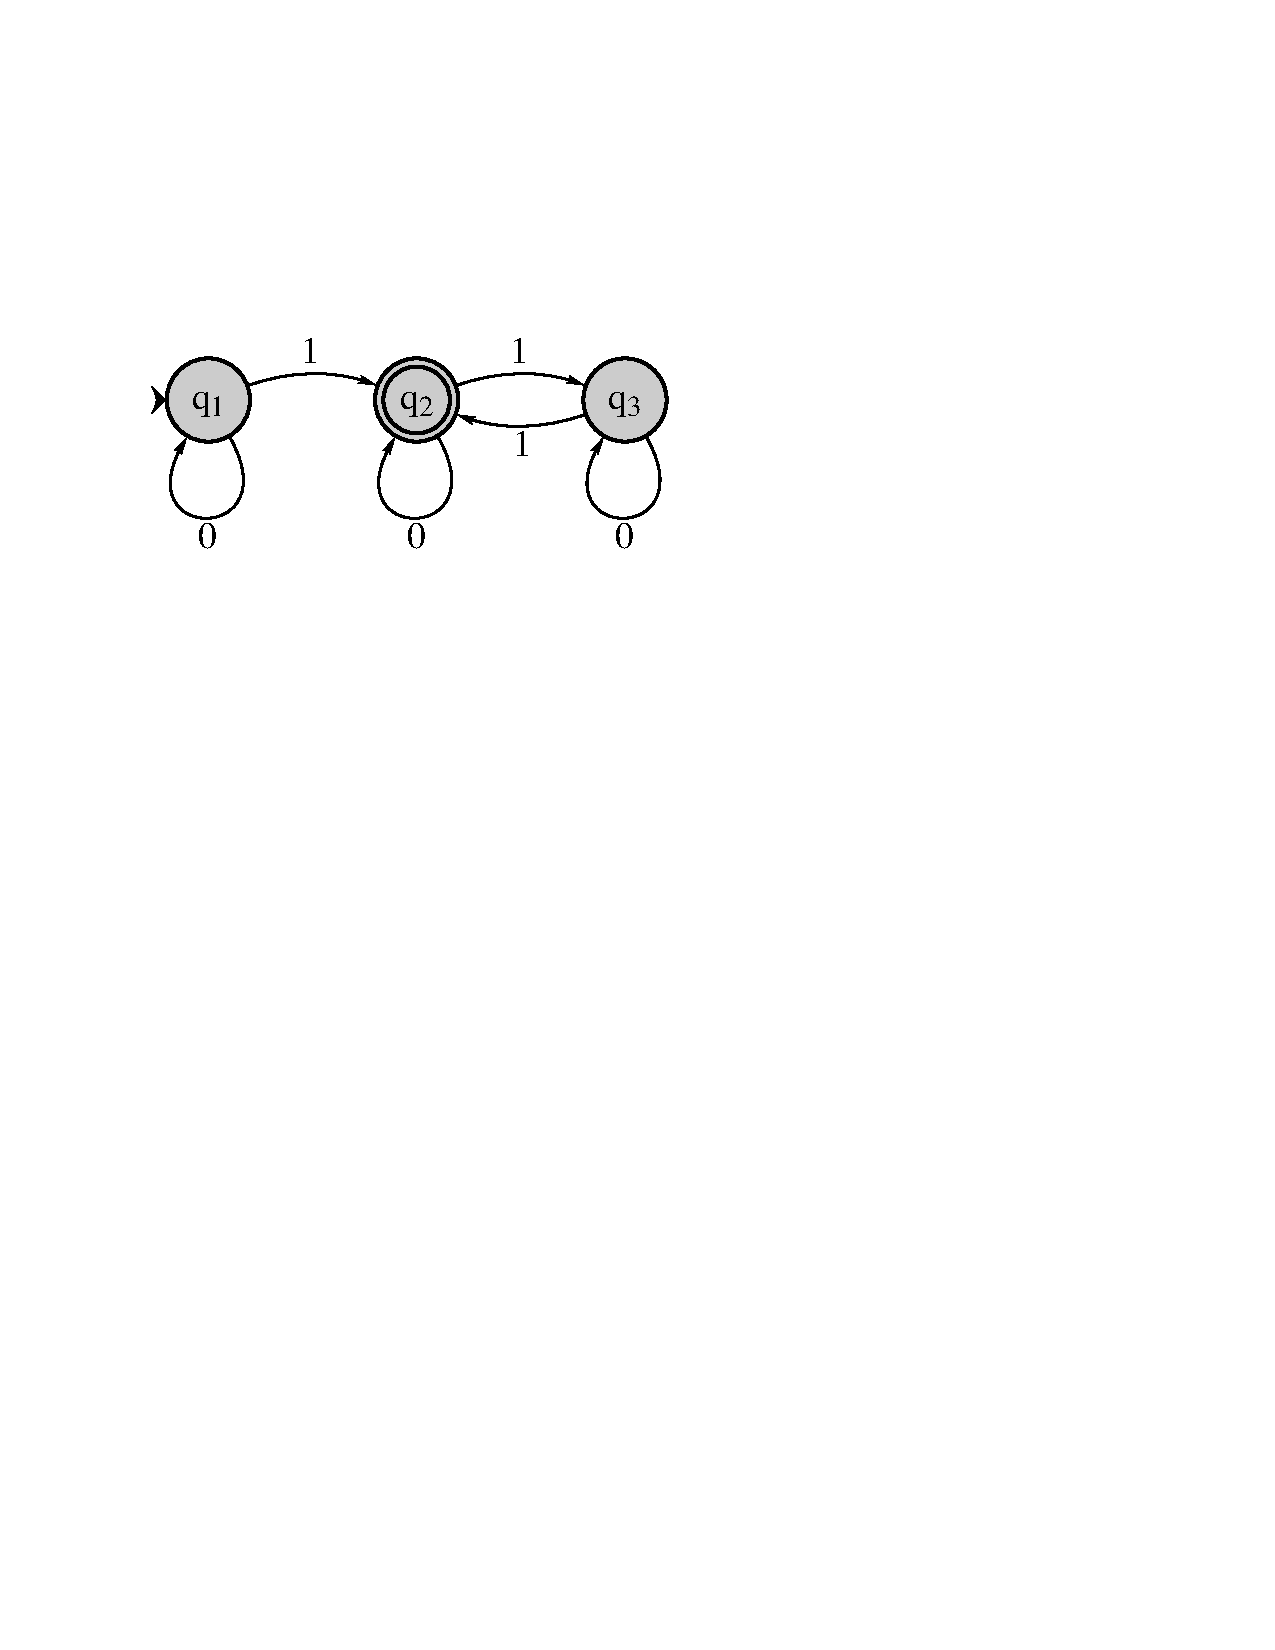
\includegraphics{automin1.pdf}}
\end{center}
\caption{A simple finite automaton}
\label{autom}
\end{figure}
         % Chapter 7, chap7.tex contains an	
                        % example of figs and tables and inclusion of pdf.

%%%%%%%%%%%%%%%%%%%%
% Concluding Pages %
%%%%%%%%%%%%%%%%%%%%%%%%%%%%%%%%%%%%%%%%%%%%%%%%%%%%%%%%%%%%%%%%%%%%%%%%%%%%%%%%

% Bibliography or References, REQUIRED

% If using bibtex, create or modify the refs.bib file
% and use (uncomment) the following three lines.
%\bibliographystyle{plain}     %You may prefer \bibliographystyle{alpha}
%\addcontentsline{toc}{chapter}{\bibname}
%\bibliography{refs}

% If using the ``thereference'' environment instead, modify the ref.tex file
% and use the following line
% ref.tex {References}

\addcontentsline{toc}{chapter}{References}
\begin{thereferences}{99}

\bibitem{Luo1992}
Luo, Z.Q. \& Tseng, P. J,
Optim Theory Appl (1992) 72: 7. doi:10.1007/BF00939948

\bibitem{Yoon2014}
@article{kim2014convolutional,
  title={Convolutional neural networks for sentence classification},
  author={Kim, Yoon},
  journal={arXiv preprint arXiv:1408.5882},
  year={2014}
}


\bibitem{Cook1971}
S.~Cook,
 ``The complexity of theorem-proving procedures,''
 {\it Proceedings of the 3rd ACM Symposium on Theory of Computing},
 Shaker Heights, Ohio, 1971, pp.~151--158.
\end{thereferences}


% If including appendices, uncomment the following lines,
% adding more includes if needed.
%\StartAppendix
%\include{AppendixA}         % Example of how to include an appendix

% vitae.tex (Curriculum Vitae)

\addcontentsline{toc}{chapter}{Curriculum Vitae}
\chapter*{Curriculum Vitae}



% The following is no longer needed when typed by the author.
%\noindent
%This thesis was typed by <name of typist>.
         % Curriculum Vitae      REQUIRED

%%%%%%%%%%%%%%%%%%%%%%%%%%%%%%%%%%%%%%%%%%%%%%%%%%%%%%%%%%%%%%%%%%%%%%%%%%%%%%%%

\end{document}
